\section{Spezielle Verteilung}
\subsection{Diskrete Verteilung}
%\subsection{Rechteckverteilung}
%$ X ~ U_{]a,b[} $; 
%$ f( x ) = \frac{1}{b-a}, a \le x \le b; 0, sonst $
%$ E[X] = \frac{a+b}{2} $; 
%$Var[x] = \frac{1}{12}( b^{2} + a^{2} - 2ab) $
\subsection{Bernouilliverteilung}
Indikatorvariable mit den Werten 1 bei Erfolg und 0 bei Misserfolg;
\textbf{Wahrscheinlichkeit:}$P(X=1) = p, P(X=0)  = 1 - p$; 
\textbf{Verteilung:} $X \thicksim B_{1,p}$ p ist Erfolgswahrscheinlichkeit; 
$E[X] = p = \sum x_{i} \cdot p(x_{i}) = 1 \cdot p(1)$; 
$Var[X] = p(1-p)  = E[X^2] -(E[X])^2 = p - p^2 = p(1-p)$; 
\subsection{Binominalverteilung}
\underline{Anzahl der Erfolge beim n-maligen Ziehen} \textbf{mit Zurücklegen};
\textbf{Wahrscheinlichkeit} $ P(x = k ) =  \binom{n}{k} \cdot p^k \cdot (1-p)^{n-k}, k \in {0, 1, ..., n}$; 
\textbf{Verteilung} $ X \thicksim B_{n, p}$; 
$E[X] = np$; 
$ Var[X] = np(1-p) $; 
\textbf{R:}
\textcolor{red}{d}binom(k,n,p)=P(X=k) $\hat{=}$Wahrscheinlichkeits-/Dichtefunktion; 
\textcolor{red}{p}binom(k,n,p)=F(k) $\hat{=}$Verteilungsfunktion; 
\textcolor{red}{q}binom(q,n,p)$\hat{=}$q-Quantil; 
\textcolor{red}{r}binom(k,n,p)$\hat{=}$kbinomialverteilte Zufallszahlen; 
\subsection{Hypergeometrische Verteilung}
Anzahl der Erfolge beim \textbf{n-maligen Ziehen ohne Zurücklegen} aus einer Menge mit M Elementen, die Erfolg bedeuten, und N Elementen, die Misserfolg bedeuten. $Gesamtumfang = M + N$;
\textbf{Wahrscheinlichkeit}
$ P(X=k) = \frac{\binom{M}{k} \cdot \binom{N}{n-k}}{\binom{M+N}{n}}, k \in \{0, 1, ..., min\{n,M\}\}$;
\textbf{Verteilung} $ X \thicksim H_{M, N, n}$; $E[X] = n \frac{M}{M+N}$; $\frac{M}{M+N} \hat{=} Trefferwahrscheinlichkeit$; $Var[X] = n \frac{M}{M+N}( 1 - \frac{M}{M+N}) \frac{M+N-n}{M+N-1}$; $\rightarrow 1$ falls n klein im Verhältnis zu M+N;
\textbf{R:}
$\textcolor{red}{d}hyper(k,M,N,n)=P(X=k)$;
$\textcolor{red}{p}hyper(k,M,N,n)=F(k)$;
Falls $ 20n \le M + N \& M + N $ groß, Unterschied zw. "Ziehen ohne bzw. mit Zurücklegen" unwesentlich, es kann die Binomialverteilung mit $ p = \frac{M}{M+N} $ als Approximation für die hypergeom. Vert. verwendet werden.
\subsection{Poisson-Verteilung}
\textbf{Verteilung der seltenen Ereignisse} Häufigkeit punktförmiger Ereignisse in einem Kontinuum. Die durchschnittlich zu erwartende Anzahl der Erfolge $\lambda$ pro Maßeinheit (i. a. Zeiteinheit) sei bekannt. $k \in \mathbb{N}_{0} \rightarrow diskret$
\textbf{Wahrscheinlichkeit}$P (X = k) = \frac{\lambda^k}{k!}e^{-\lambda}$ mit $ \sum_{k=0}^{\infty} P(X=k) = 1, da \sum_{k=0}^{\infty} \frac{\lambda^k}{k!} = e^{\lambda}$; 
\textbf{Verteilung} $X \thicksim P_{\lambda}$; 
$E[X] = \lambda, da \sum_{k=0}^{\infty} k\frac{\lambda^k}{k!} e^{-\lambda} = e^{-\lambda}\sum_{k=1}^{\infty}\lambda \frac{\lambda^{k-1}}{(k-1)!} = \lambda e^{-\lambda} \sum_{i=0}^{\infty} \frac{\lambda^i}{i!} = \lambda$; 
$Var[X] = \lambda$ 
\textbf{R:} 
$\textcolor{red}{d}pois(k,\lambda)=P(X=k)$; 
$\textcolor{red}{p}pois(k,\lambda)=F(k)$; 
$ \lambda $ = np.
\subsection{Gleichverteilung}
Alle Werte $\{x_{1},...,x_{n}\}$einer ZV X sind gleich wahrscheinlich; 
\textbf{Wahrscheinlichkeit} 
$P(X=x_{k}) = \frac{1}{n}$; 
\textbf{Verteilung} 
$X \thicksim U_{\{x_{1}, ..., x_{n}\}}$; 
$E[X] = \frac{1}{n} \sum_{k=1}^{n} x_{k} = \overline{x}$; 
$Var[X] = \frac{1}{n} \sum_{k=1}^{n} x_{k}^2 - \overline{x}^2$; 
\textbf{R:} 
$sample(1:N,n) \hat{=}$ n Zufallszahlen zwischen 1 und N
\subsection{Stet.Vert.}
\subsection{Gleichverteilung/Rechteck}
Zufallszahlen aus einem Intervall $[a,b]$; 
\textbf{Dichte:} 
$f(x) = \frac{1}{b-a}$ für $x \in [a,b]$; 
\textbf{Verteilung:} 
$X \thicksim U_{[a,b]}$; 
$E[X] = \frac{a+b}{2}$; 
$Var[X] = \frac{(b-a)^2}{12}$
\textbf{R:} 
$\textcolor{red}{d}unif(x,a,b)=f(x)$; 
$\textcolor{red}{p}unif(x,a,b)=F(x)$; 
$\textcolor{red}{r}unif(n) \hat{=}$ n Zufallszahlen zwischen 0 und 1; 
$\textcolor{red}{r}unif(n, a, b) \hat{=}$ n Zufallszahlen zwischen a und b; 
\subsection{Normalverteilung}
Beschreibt viele reale Situationen, ist insbesondere Grenzverteilung unabhängiger Summen; 
\textbf{Dichte:} 
$f(x) = \frac{1}{\sigma\sqrt{2\pi}}e^{(-\frac{1}{2}(\frac{x-\mu}{\sigma})^2)}$; 
\textbf{Verteilung:} 
$X \thicksim N_{\mu, \sigma^2} $; 
$E[X] = \mu $; 
$Var[X] = \sigma^2 $; 
\textbf{R:} 
$\textcolor{red}{d} norm(x,\mu,\textcolor{red}{\sigma})=f(x) $; 
$\textcolor{red}{p} norm(x,\mu,\textcolor{red}{\sigma})=F(x) $; 
$\textcolor{red}{q} norm(q,\mu,\textcolor{red}{\sigma}):q-Quantil $; 
\textbf{Maximalstelle} von $ f(x) $ bei $ x =\mu $; 
\textbf{Wendestelle} von $ f(x) $ bei $ x = \mu \pm \sigma $; 
$ E[aX + b] = aE[X] + b $; 
$ Var [aX + b] = a^2 Var[X] $; 
$ X \thicksim N_{\mu, \sigma^2} \Rightarrow aX + b \thicksim N_{a\mu+b, a^2\sigma^2}$ und 
\underline{Z-Trafo:} $ \frac{X-\mu}{\sigma} \thicksim N_{0,1} $; 
$ X_ {1} \thicksim N_{\mu_{1}, \sigma_{1}^2}$ und $ X_{2} \thicksim N_{\mu_{2}, \sigma_{2}^2} \underbrace{\Rightarrow} X_{1} + X_{2} \thicksim N_{ \mu_{1} + \mu_{2}, \sigma_{1}^2 + \sigma_{2}^2} $;\\
$ X_{1}, X_{2} $ stochastisch unabhängig
\subsection{Standardnormalverteilung}
\textbf{Dichte:} 
$\varphi(x) = \frac{1}{\sqrt{2}}e^{(-\frac{1}{2}x^2)} $; 
\textbf{Verteilung}
$\phi(x) = \int_{-\infty}^{x} \varphi (t) dt$; 
\textbf{Quantile:} 
$ \phi (-x) = 1 - \phi (x) \Rightarrow -x_{p} = x_{1-p} $ z.B. 
$ -x_{0.25} = x_{0.75} $; 

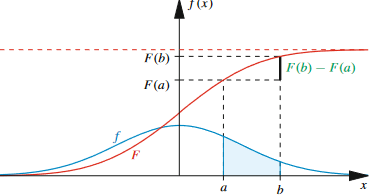
\includegraphics[scale=0.3]{./pic/fFxcombined.png}
%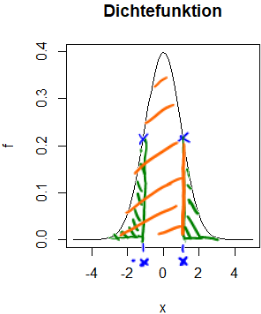
\includegraphics[scale=0.3]{./pic/NormalverteilungDichtefunktion.png}
%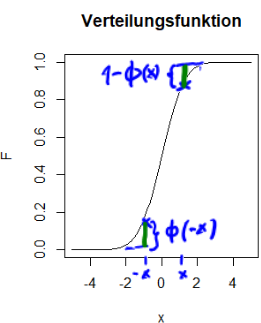
\includegraphics[scale=0.3]{./pic/NormalverteilungVerteilungsfunktion.png}
\textbf{Schätzwerte:}
$ Z = \frac{x-\mu}{\sigma} \thicksim N_ {0,1}$; 
$ P( \mu -\sigma \le X \le \mu + \sigma) = P ( -1 \le Z \le 1 ) \approx 68\% $; 
$ P ( \mu -2\sigma \le X \le \mu +2\sigma ) = P( -2 \le Z \le 2 ) \approx 95\% $; 
$ P( \mu - 3 \sigma \le X \le \mu + 3\sigma) = P ( -3 \le Z \le 3 ) \approx 99.7\% $
\subsection{Exponentialverteilung}
Modellierung von Lebensdauern, Wartezeiten Sei $ Y_{t} \thicksim P_{\lambda t} $ im Intervall $ [0,t] $  von $ t $  Zeiteinheiten, dann beschreibt die Exponentialverteilung die Wartezeit $ X $ bis zum Eintreten eines Ereignisses; 
\textbf{Dichte- und Verteilungsfunktion:} 
$ f(x) = \lambda e^{-\lambda x} (x \ge 0) $ und 
$ F(x) = 1 - e^{-\lambda x}$; 
\textbf{Verteilung:} 
$ X \thicksim Exp_{\lambda}$; 
$ E[X] = \frac{1}{\lambda} \Rightarrow$ Berechnung mit partieller Integration; 
$ Var[X] = \frac{1}{\lambda^2}$;
\textbf{R:} 
$ \textcolor{red}{d}exp(x,\lambda) = f(x)$; 
$ \textcolor{red}{p}exp(x,\lambda) = F(x)$; 
\textbf{Eigenschaft:} 
Eine exponentialverteile ZV X ist gedächtnislos, d.h. 
$ P(X > s + t) | X > t = P( X > s)$; 
gl. Vert.
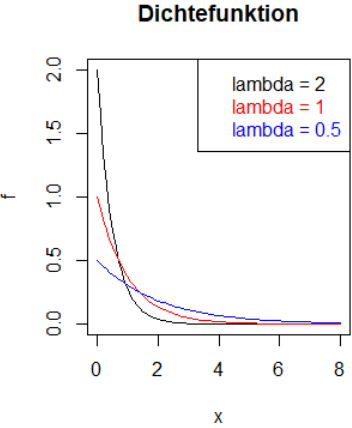
\includegraphics[scale=0.25]{./pic/ExponentialverteilungDichtefunktion.png}
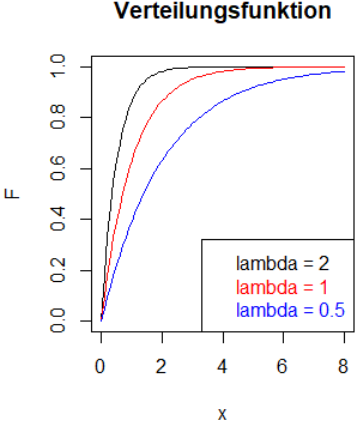
\includegraphics[scale=0.25]{./pic/ExponentialverteilungVerteilungsfunktion.png}
\subsection{Chiquadrat-Verteilung}
$ Z_{1},...,Z_{n}$ seien unabhängige, standardnormalverteilte ZV $\Rightarrow  X=Z_{1}^2+···+Z_{n}^2 $ hat Chiquadratverteilung mit n Freiheitsgraden;
\textbf{Anwendungsmodell:} 
Summen unabhängiger, standardnormalverteilter ZV;
\textbf{Verteilung:} 
$ X \thicksim  \chi_{n}^2$; 
$ E[X] = n $; 
$ Var[X] = 2n $; 
\textbf{R:} 
$ \textcolor{red}{d} chisq(x,n)=f(x)$; 
$\textcolor{red}{p} pchisq(x,n)=F(x)$; 
\textbf{Eigenschaft:} 
$ X_{1} \thicksim \chi_{n1}^2 $ und $ X_{2} \thicksim \chi_{2}^2 \Rightarrow X_{1} + X_{2} \thicksim \chi_{n_{1} + n_{2}} $
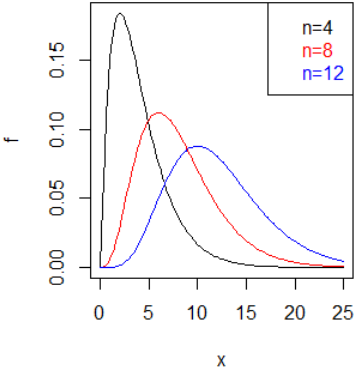
\includegraphics[scale=0.25]{./pic/Chiquadratverteilung.png}
\subsection{t-Verteilung}
$ Z \thicksim N_{0,1} $ und $ X \thicksim \chi_{n}^2 \Rightarrow Y = \frac{Z}{\frac{X}{\sqrt{n}}} $ ist t-verteilt mit n Freiheitsgraden; 
\textbf{Anwendungsmodell:}
Schätz- und Testverfahren bei unbekannter Varianz; 
\textbf{Verteilung:} 
$ Y \thicksim t_{n} $; 
$ E[Y] = 0  $ für $ n > 1 $; 
$ Var[Y] = \frac{n}{n-2} $ für $ n > 2 $; 
\textbf{R:} 
$\textcolor{red}{d}t(y,n) \hat{=} f(x) $; 
$ \textcolor{red}{p}t(y,n) \hat{=} F(x)$; 
$ \textcolor{red}{q}t(y, n) \hat{=} F^{-1}(x)$; 
\textbf{Eigenschaften:} 
Für $ n  \rightarrow \infty : t_{n} \rightarrow N_{0,1}$; 
Achsensymmetrie der Dichtefunktion $ \Rightarrow -y_{p} = x_{1-p} $
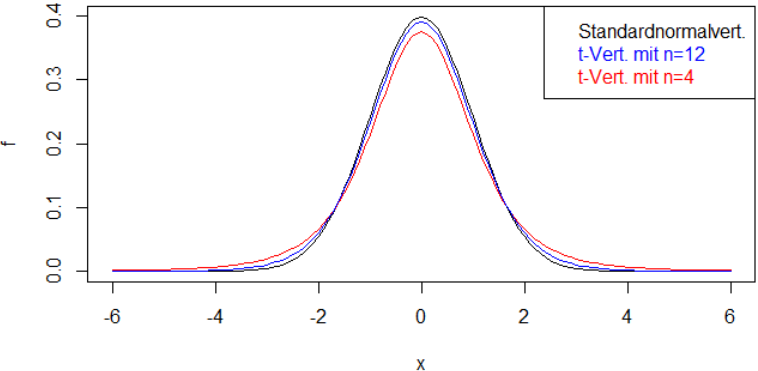
\includegraphics[scale=0.25]{./pic/t-Verteilung.png}\\
Abbildung Dichtefunktion